\chapter{Whole-Genome and Exome Sequencing}
\label{ch:genomeseq}

The ability to read the complete DNA sequence of an organism---or strategically selected portions of it---has transformed biology, medicine, and agriculture. In this chapter, we explore the three major strategies for interrogating genomic DNA: \textbf{whole-genome sequencing (WGS)}, which captures every nucleotide from telomere to telomere; \textbf{whole-exome sequencing (WES)}, which focuses on the protein-coding regions; and \textbf{targeted gene panels}, which zoom in on a curated set of genes relevant to a specific clinical question. We examine the technical workflows, compare the trade-offs of each approach, and build complete analysis pipelines in both Snakemake and Nextflow.

%% ============================================================
\section{Whole-Genome Sequencing (WGS)}
\label{sec:wgs}
%% ============================================================

\subsection{What WGS Captures}

Whole-genome sequencing aims to determine the nucleotide sequence of an organism's \emph{entire} genome. For the human genome, this means approximately 3.1 billion base pairs distributed across 22 autosomes and two sex chromosomes, plus the 16.6\kilobase{} mitochondrial genome. Critically, WGS captures:

\begin{itemize}[nosep]
  \item \textbf{Protein-coding exons} ($\sim$1.5\% of the genome, $\sim$20,000 genes).
  \item \textbf{Non-coding regulatory elements}: promoters, enhancers, silencers, insulators, and super-enhancers that control when, where, and how much a gene is expressed.
  \item \textbf{Intronic sequences}: including splice-regulatory elements and deeply intronic variants that can create cryptic exons.
  \item \textbf{Intergenic regions}: harbouring long non-coding RNA (lncRNA) genes, microRNA genes, and disease-associated variants identified by GWAS.
  \item \textbf{Repetitive elements}: transposable elements (SINEs, LINEs, LTRs), tandem repeats (microsatellites, minisatellites), segmental duplications, and centromeric/telomeric satellite DNA.
  \item \textbf{Structural variation}: large deletions, duplications, inversions, and translocations that are invisible to exome-only approaches.
  \item \textbf{Mitochondrial DNA}: enabling studies of heteroplasmy, maternal lineage, and mitochondrial disease.
\end{itemize}

\begin{keyconcept}[title={Why the Non-Coding Genome Matters}]
Although only $\sim$1.5\% of the human genome encodes proteins, the ENCODE project demonstrated that $\sim$80\% shows biochemical activity. Over 90\% of disease-associated variants from GWAS fall in non-coding regions. WGS is the only unbiased approach that captures all of these elements.
\end{keyconcept}

\subsection{When to Use WGS vs.\ Targeted Approaches}

The decision of whether to perform WGS, WES, or a targeted panel depends on the scientific question, budget, required depth, and turnaround time. \Cref{tab:wgs_vs_wes_vs_panel} provides a detailed comparison. In general:

\begin{itemize}[nosep]
  \item \textbf{Use WGS} when you need a comprehensive, unbiased view of the genome---for example, in rare disease cases where WES was negative, cancer whole-genome analysis, structural variant detection, population genomics, or de novo genome assembly.
  \item \textbf{Use WES} when the primary question concerns protein-coding variants, particularly for Mendelian disease diagnostics where cost efficiency matters.
  \item \textbf{Use targeted panels} when a well-defined set of genes is associated with the phenotype (e.g., oncology panels, pharmacogenomics panels) and ultra-deep coverage is required for detecting low-frequency variants.
\end{itemize}

\subsection{Sequencing Depth Requirements}
\label{subsec:depth}

Sequencing depth (also called coverage) is the average number of times each base in the genome is read. The required depth depends on the application:

\begin{itemize}[nosep]
  \item \textbf{Germline variant calling}: 30$\times$ is the community standard for high-confidence SNV and indel detection in diploid genomes. The Genome in a Bottle Consortium validated this threshold extensively.
  \item \textbf{Somatic/cancer sequencing}: 60--100$\times$ for tumor samples (paired with $\sim$30--40$\times$ for the matched normal) to reliably detect subclonal mutations at variant allele frequencies (VAF) as low as 5--10\%.
  \item \textbf{Ultra-deep cancer sequencing}: 500--1000$\times$ or more for detecting rare subclonal variants or circulating tumor DNA (ctDNA) in liquid biopsies.
  \item \textbf{De novo assembly}: 30--50$\times$ HiFi long reads, supplemented by 60--100$\times$ ultra-long Oxford Nanopore reads for scaffolding.
  \item \textbf{Population-scale studies}: As low as 4--10$\times$ with imputation (e.g., the TOPMed and All of Us programs) to reduce per-sample cost while maintaining statistical power at the cohort level.
\end{itemize}

\begin{warningbox}[title={Low-Pass WGS Limitations}]
Low-pass WGS ($<$10$\times$) is cost-effective for large population studies when combined with genotype imputation, but it is \emph{not} suitable for clinical variant calling in individual patients. Individual genotype calls at low depth have high error rates, and rare variants unique to a single individual cannot be imputed.
\end{warningbox}

\subsection{Short-Read WGS Workflow}

The canonical short-read WGS workflow proceeds through the following stages:

\begin{enumerate}[nosep]
  \item \textbf{Library preparation}: Genomic DNA is extracted, fragmented (enzymatic or mechanical), end-repaired, A-tailed, and ligated to platform-specific adapters. PCR amplification (typically 4--8 cycles) or PCR-free protocols are used. PCR-free libraries reduce amplification bias and are preferred for WGS.
  \item \textbf{Sequencing}: Libraries are loaded onto the sequencing instrument (e.g., Illumina NovaSeq X, AVITI by Element Biosciences). Paired-end 150\basepair{} reads are standard for WGS.
  \item \textbf{Quality control}: Raw FASTQ files are assessed with \software{FastQC} and \software{MultiQC}. Adapter trimming and quality filtering are performed with \software{fastp} or \software{Trimmomatic}.
  \item \textbf{Alignment}: Trimmed reads are mapped to the reference genome using \software{BWA-MEM2} (or the original \software{BWA-MEM}) for short reads. The output is a sorted BAM/CRAM file.
  \item \textbf{Duplicate marking}: PCR duplicates are flagged with \software{sambamba markdup}, \software{Picard MarkDuplicates}, or \software{biobambam2}.
  \item \textbf{Base quality score recalibration (BQSR)}: GATK's \software{BaseRecalibrator} adjusts quality scores using known variant sites (dbSNP, Mills indels).
  \item \textbf{Variant calling}: Germline variants are called with \software{GATK HaplotypeCaller} or \software{DeepVariant}. Structural variants are called with \software{Manta}, \software{DELLY}, or \software{Smoove}.
  \item \textbf{Variant filtering and annotation}: Variants are filtered (VQSR or hard filters) and annotated with \software{VEP}, \software{SnpEff}, or \software{ANNOVAR}.
\end{enumerate}

\begin{protocolbox}[title={PCR-Free vs.\ PCR-Based WGS Libraries}]
\textbf{PCR-free libraries} are the gold standard for WGS because they:
\begin{itemize}[nosep]
  \item Eliminate PCR duplicate reads, increasing effective coverage.
  \item Reduce GC-composition bias, improving uniformity across AT-rich and GC-rich regions.
  \item Improve coverage of repetitive regions.
  \item Require higher DNA input ($\sim$100--500\,ng) compared to PCR-based protocols ($\sim$1--50\,ng).
\end{itemize}
Use PCR-based protocols only when input DNA is limiting (e.g., clinical FFPE samples, forensic samples).
\end{protocolbox}

\subsection{Long-Read WGS}

Long-read sequencing technologies from PacBio (HiFi reads, 10--25\kilobase{} at $>$Q30 accuracy) and Oxford Nanopore Technologies (ultra-long reads exceeding 100\kilobase{}, some $>$1\megabase{}) provide critical advantages for WGS:

\begin{itemize}[nosep]
  \item \textbf{Structural variant detection}: Long reads span breakpoints of deletions, duplications, inversions, and translocations that are invisible to short reads due to repetitive flanking sequences.
  \item \textbf{Haplotype phasing}: Reads that span multiple heterozygous variants enable direct physical phasing of alleles across kilobases to megabases.
  \item \textbf{Repeat characterisation}: Tandem repeat expansions (e.g., \gene{FMR1} CGG repeats in Fragile X, \gene{HTT} CAG repeats in Huntington's disease, \gene{C9orf72} GGGGCC repeats in ALS/FTD) can be directly measured.
  \item \textbf{Methylation detection}: Nanopore sequencing natively detects 5-methylcytosine (5mC) and other base modifications without bisulfite conversion.
  \item \textbf{De novo assembly}: Long reads are essential for resolving repetitive regions and producing highly contiguous genome assemblies.
\end{itemize}

\begin{tipbox}[title={Combining Short and Long Reads}]
A hybrid approach using 30$\times$ short-read Illumina data plus 30$\times$ PacBio HiFi data provides the best of both worlds: the cost-effective SNV/indel accuracy of short reads and the structural variant resolution and phasing of long reads. This is increasingly being adopted in clinical rare disease programs.
\end{tipbox}

\subsection{De Novo Genome Assembly}
\label{subsec:denovo}

De novo genome assembly is the process of reconstructing a genome sequence without a reference. This is essential for non-model organisms, population-specific reference construction, and resolving complex genomic regions that collapse in reference-based analyses.

\subsubsection{Assembly Concepts}

\begin{description}[style=nextline]
  \item[Contigs] Contiguous sequences assembled from overlapping reads. A contig has no gaps.
  \item[Scaffolds] Ordered and oriented contigs linked by paired-end or long-range information (mate-pair reads, Hi-C, optical mapping), with gaps represented as stretches of N characters.
  \item[N50] The length $N$ such that 50\% of the total assembly size is contained in contigs (or scaffolds) of length $\geq N$. Higher N50 indicates a more contiguous assembly. Note: N50 alone does not measure \emph{correctness}.
  \item[NG50] Like N50, but normalised to the expected genome size rather than the assembly size. Prevents inflated N50 from incomplete assemblies.
  \item[BUSCO completeness] Benchmarking Universal Single-Copy Orthologs---measures the fraction of expected single-copy genes present in the assembly. A complete genome should have $>$95\% BUSCO completeness.
  \item[QV (consensus quality)] The Phred-scaled accuracy of the consensus sequence. QV50 means one error per 100,000 bases; QV60 means one error per 1,000,000 bases.
\end{description}

\subsubsection{Modern Assembly Approaches}

Current best-practice de novo assembly combines multiple data types:

\begin{enumerate}[nosep]
  \item \textbf{PacBio HiFi assembly}: Tools such as \software{hifiasm} produce highly accurate, haplotype-resolved assemblies from HiFi reads alone.
  \item \textbf{Ultra-long ONT reads}: Reads $>$100\kilobase{} span centromeric satellites, segmental duplications, and other complex repeats. \software{Verkko} and \software{hifiasm} (with ONT integration) use these to connect HiFi contigs.
  \item \textbf{Hi-C scaffolding}: Chromatin conformation data provides chromosome-scale scaffolding. Tools: \software{YaHS}, \software{SALSA2}, \software{3D-DNA}.
  \item \textbf{Polishing}: Consensus accuracy is refined using \software{DeepConsensus} (PacBio), \software{Medaka} (ONT), or short-read polishing with \software{Pilon} or \software{Merqury}-guided assessment.
\end{enumerate}

\subsubsection{De Bruijn Graph Formalism}
\label{subsubsec:genomeseq:debruijn}

Most modern short-read assemblers---including \software{SPAdes}, \software{MEGAHIT}, and the local assembly module within \software{GATK HaplotypeCaller}---are founded on \textbf{de Bruijn graphs}. Understanding this formalism is essential for interpreting assembly behaviour and diagnosing failures.

\begin{keyconcept}[title={Definition of a de Bruijn Graph}]
Given a set of reads and a fixed integer $k$, the de Bruijn graph $G_k = (V, E)$ is a directed graph defined as follows:
\begin{itemize}[nosep]
  \item \textbf{Nodes} $V$: Every unique $(k{-}1)$-mer observed in the read set.
  \item \textbf{Edges} $E$: For each $k$-mer $s_1 s_2 \cdots s_k$ in the reads, a directed edge connects the $(k{-}1)$-mer prefix $s_1 \cdots s_{k-1}$ to the $(k{-}1)$-mer suffix $s_2 \cdots s_k$.
\end{itemize}
The genome reconstruction problem reduces to finding a path through this graph that traverses every \emph{edge} exactly once---an \textbf{Eulerian path}.
\end{keyconcept}

A connected directed graph possesses an Eulerian path if and only if (i) it is connected (considering the underlying undirected graph) and (ii) at most two nodes have unequal in-degree and out-degree. When these conditions hold, the walk can be computed in $O(|E|)$ time using Hierholzer's algorithm. In practice, sequencing errors, polymorphisms, and repeats introduce branches, tips, and bubbles that must be resolved by heuristic graph simplification.

\paragraph{Choice of $k$: the sensitivity--specificity trade-off.}
The parameter $k$ profoundly affects assembly quality:

\begin{itemize}[nosep]
  \item \textbf{Small $k$} increases \emph{sensitivity}: more $k$-mers survive the read error filter, producing a more connected graph. However, many distinct genomic loci share the same short $k$-mer, collapsing repeats and creating ambiguous paths.
  \item \textbf{Large $k$} increases \emph{specificity}: $k$-mers are more likely to be unique in the genome, resolving repeats and reducing spurious edges. However, $k$-mers that span sequencing errors are lost, fragmenting the graph.
\end{itemize}

The number of distinct $k$-mers in a genome of size $G$ is bounded by:
\begin{equation}
\label{eq:genomeseq:kmers}
N_k \leq \min\!\bigl(G - k + 1,\; 4^k\bigr),
\end{equation}
where $4^k$ is the total number of possible $k$-mers over the DNA alphabet $\{A,C,G,T\}$. For the human genome ($G \approx 3.1 \times 10^9$), $k = 17$ yields $4^{17} \approx 1.7 \times 10^{10} > G$, so most 17-mers are unique; for $k = 11$, $4^{11} \approx 4.2 \times 10^6 \ll G$, meaning extensive $k$-mer collisions are inevitable. Multi-$k$ assemblers (e.g., \software{SPAdes}) iteratively build graphs at increasing $k$ values to combine the connectivity of small $k$ with the specificity of large $k$.

\begin{tipbox}[title={Practical $k$-mer Selection Rules}]
For Illumina 150\basepair{} paired-end data, $k$ values in the range 21--77 are typical. As a rule of thumb, $k$ should be (i) odd (to avoid palindromic $k$-mers), (ii) shorter than the read length, and (iii) large enough that $4^k \gg G$. Tools such as \software{KMC3} and \software{Jellyfish2} enable rapid $k$-mer counting to assess the $k$-mer spectrum before assembly.
\end{tipbox}

\paragraph{Repeat resolution strategies.}
Repeats longer than $k - 1$ bases collapse into the same graph path, creating ambiguity. Several strategies address this:

\begin{itemize}[nosep]
  \item \textbf{Paired-end information}: Mate-pair or paired-end reads spanning a repeat connect the flanking unique sequences, enabling the assembler to thread through the correct path.
  \item \textbf{Read clouds / linked reads}: Barcoded short reads from the same long DNA molecule (10x Genomics Chromium, TELL-Seq, stLFR) provide long-range linkage without long-read sequencing.
  \item \textbf{Long reads}: HiFi and ultra-long ONT reads span most genomic repeats outright, enabling overlap-layout-consensus (OLC) or string-graph assembly that avoids the de Bruijn $k$-mer limitation entirely.
  \item \textbf{Coverage depth}: Unique regions have single-copy coverage, whereas collapsed repeats exhibit proportionally elevated coverage. Assemblers exploit this signal to estimate repeat copy number.
\end{itemize}

\subsubsection{Assembly Quality Metrics: Formal Definitions}
\label{subsubsec:genomeseq:assembly_metrics}

While N50 and NG50 were introduced informally above, their precise mathematical definitions are essential for rigorous benchmarking.

Let an assembly consist of $n$ contigs with lengths $l_1 \geq l_2 \geq \cdots \geq l_n$, and let $G$ denote the known or estimated genome size.

\begin{description}[style=nextline]
  \item[N50] The contig length $L$ such that the sum of lengths of all contigs with $l_i \geq L$ constitutes at least half the total assembly size:
    \begin{equation}
    \label{eq:genomeseq:n50}
    \text{N50} = L \quad \text{where} \quad \sum_{i:\, l_i \geq L} l_i \;\geq\; \frac{1}{2}\sum_{j=1}^{n} l_j.
    \end{equation}
  \item[NG50] Identical to N50, but the denominator is the expected genome size $G$ rather than the assembly size:
    \begin{equation}
    \label{eq:genomeseq:ng50}
    \text{NG50} = L \quad \text{where} \quad \sum_{i:\, l_i \geq L} l_i \;\geq\; \frac{G}{2}.
    \end{equation}
    NG50 penalises incomplete assemblies, which may have artificially inflated N50 values.
  \item[auN (area under the Nx curve)] A single statistic that captures the entire contiguity distribution rather than a single percentile. It is defined as:
    \begin{equation}
    \label{eq:genomeseq:aun}
    \mathrm{auN} = \frac{\sum_{i=1}^{n} l_i^2}{\sum_{i=1}^{n} l_i} = \frac{\sum_{i=1}^{n} l_i^2}{A},
    \end{equation}
    where $A = \sum_i l_i$ is the total assembly length. Intuitively, auN is the expected contig length at a randomly chosen assembled base. It avoids the arbitrariness of the 50\% threshold and is increasingly preferred for benchmarking.
\end{description}

\begin{warningbox}[title={Contiguity Is Not Correctness}]
N50, NG50, and auN measure \emph{contiguity} only. A highly contiguous but mis-assembled genome (e.g., with chimeric joins) will have inflated metrics. Always complement contiguity statistics with \emph{correctness} metrics: BUSCO completeness, QV estimated by \software{Merqury}, and reference-based mis-assembly counts from \software{QUAST}.
\end{warningbox}

\subsubsection{Scaffolding Algorithms}
\label{subsubsec:genomeseq:scaffolding}

Scaffolding bridges gaps between contigs by ordering and orienting them using long-range linkage information. Three major data types are used:

\begin{description}[style=nextline]
  \item[Hi-C] Chromatin conformation capture generates read pairs from DNA fragments that were spatially proximal in the nucleus. Because contact probability decays as a power law with genomic distance ($P_{\text{contact}} \propto d^{-\gamma}$, with $\gamma \approx 1$ for mammalian genomes), Hi-C links contigs across megabase scales and assigns them to chromosomes. Tools: \software{YaHS}, \software{SALSA2}, \software{3D-DNA}, \software{ALLHiC} (for polyploid genomes).
  \item[Linked reads] Technologies such as 10x Genomics Chromium, TELL-Seq, and stLFR attach a shared barcode to short reads derived from the same $\sim$50--100\kilobase{} DNA molecule. Barcode co-occurrence connects contigs separated by up to $\sim$100\kilobase{}. Tools: \software{scaff10x}, \software{Tigmint} (mis-assembly detection), \software{Arcs}.
  \item[Optical maps] Bionano optical mapping generates restriction-enzyme--site patterns along megabase-length single molecules. These patterns are aligned to assembled contigs, enabling gap sizing and scaffolding across repeats invisible to sequence-based methods. Tools: \software{Bionano Solve}, \software{OMTools}.
\end{description}

\begin{tipbox}[title={Combining Multiple Scaffolding Data Types}]
The highest-contiguity assemblies integrate all available evidence. A common strategy: (1) assemble HiFi reads with \software{hifiasm}, (2) scaffold with linked-read data or ultra-long ONT reads, (3) apply Hi-C scaffolding to achieve chromosome-scale, and (4) validate with optical maps. The VGP (Vertebrate Genomes Project) pipeline exemplifies this multi-layered approach.
\end{tipbox}

\subsection{Telomere-to-Telomere (T2T) Assemblies}

The Telomere-to-Telomere (T2T) Consortium achieved a landmark in 2022 by completing the first gapless human genome assembly, T2T-CHM13. This filled $\sim$200\megabase{} of previously unresolved sequence, including:

\begin{itemize}[nosep]
  \item All 22 autosomal centromeres (arrays of $\alpha$-satellite repeats).
  \item The five acrocentric short arms (chromosomes 13, 14, 15, 21, 22) containing ribosomal DNA arrays.
  \item Telomeric repeats (TTAGGG)$_n$ at all chromosome ends.
  \item Segmental duplications that collapsed in previous assemblies.
  \item 99 previously unannotated protein-coding genes.
\end{itemize}

The T2T assembly was achieved using a combination of PacBio HiFi reads ($\sim$30$\times$), Oxford Nanopore ultra-long reads ($\sim$120$\times$), and Hi-C data, applied to the CHM13 hydatidiform mole cell line (which is nearly homozygous, simplifying assembly).

\begin{keyconcept}[title={The Evolution of Human Reference Genomes}]
\begin{description}[nosep,style=nextline]
  \item[GRCh37/hg19 (2009)] The workhorse reference for a decade. Still used in many legacy clinical databases.
  \item[GRCh38/hg38 (2013)] Improved representation of centromeres, added alternate loci (ALT contigs). The current standard for most clinical and research pipelines.
  \item[T2T-CHM13 (2022)] The first truly complete human genome. No gaps, no unresolved regions. Increasingly adopted for research, but clinical adoption is ongoing.
  \item[Human Pangenome Reference (2023--)] A graph-based reference incorporating genetic diversity from hundreds of individuals. Reduces reference bias and improves variant calling in diverse populations. Built using \software{Minigraph-Cactus} and \software{PGGB}.
\end{description}
\end{keyconcept}

\subsection{Clinical WGS}

WGS has entered clinical practice in several domains:

\begin{itemize}[nosep]
  \item \textbf{Rare disease diagnosis}: WGS achieves diagnostic yields of 25--40\% in previously undiagnosed cases, outperforming WES (which yields $\sim$25--30\%). The improvement comes from detecting non-coding variants, structural variants, and repeat expansions.
  \item \textbf{Pharmacogenomics}: WGS comprehensively genotypes pharmacogenes (CYP2D6, CYP2C19, CYP3A5, DPYD, TPMT, etc.), including complex structural variants like CYP2D6 gene deletions and duplications.
  \item \textbf{Rapid WGS in NICU/PICU}: Ultra-rapid WGS ($<$24 hours from blood draw to diagnosis) has been implemented for critically ill neonates, achieving diagnostic rates of $\sim$30--40\% and changing clinical management in $\sim$70\% of diagnosed cases.
  \item \textbf{Cancer whole-genome sequencing}: Programmes such as the UK's 100,000 Genomes Project and Hartwig Medical Foundation have demonstrated the clinical utility of tumor/normal WGS for treatment selection.
\end{itemize}

%% ============================================================
\section{Whole-Exome Sequencing (WES)}
\label{sec:wes}
%% ============================================================

\subsection{What the Exome Is}

The exome comprises the protein-coding regions (exons) of all known genes. In the human genome:

\begin{itemize}[nosep]
  \item There are approximately 20,000 protein-coding genes.
  \item The total target region is approximately 30--60\megabase{}, depending on the capture kit and whether UTRs (untranslated regions) and miRNA genes are included.
  \item This represents roughly 1--2\% of the total genome.
  \item Despite its small size, the exome harbours approximately 85\% of known disease-causing mutations (as catalogued in ClinVar and HGMD).
\end{itemize}

\subsection{Hybridisation Capture Workflow}

WES uses hybridisation capture (also called hybrid capture or target enrichment) to selectively enrich exonic sequences:

\begin{enumerate}[nosep]
  \item \textbf{Library preparation}: Standard WGS library prep---fragmentation, end-repair, adapter ligation, PCR amplification.
  \item \textbf{Hybridisation}: The library is incubated with biotinylated oligonucleotide probes (baits) complementary to exonic targets. Hybridisation occurs in solution (liquid-phase capture) over 4--16 hours.
  \item \textbf{Capture}: Streptavidin-coated magnetic beads bind the biotinylated probes and their hybridised library fragments. Non-target fragments are washed away.
  \item \textbf{Amplification}: Captured fragments undergo PCR amplification (8--12 cycles) to generate sufficient material for sequencing.
  \item \textbf{Sequencing}: Paired-end 150\basepair{} reads on Illumina platforms, targeting 80--150$\times$ mean coverage on target.
\end{enumerate}

\begin{warningbox}[title={WES Uniformity Challenges}]
Hybridisation capture is inherently non-uniform. Some exons are captured efficiently while others are poorly represented due to:
\begin{itemize}[nosep]
  \item Extreme GC content (very AT-rich or GC-rich regions).
  \item Repetitive sequences flanking target exons.
  \item Pseudogene interference (probes cross-hybridise to homologous pseudogene sequences).
  \item Probe design gaps in newly annotated genes.
\end{itemize}
Typically, 80--90\% of target bases achieve $\geq$20$\times$ coverage, but some clinically important exons may be consistently undercovered.
\end{warningbox}

\subsection{When WES Is Preferred over WGS}

\begin{itemize}[nosep]
  \item \textbf{Cost}: WES costs approximately one-third to one-quarter of WGS, making it attractive for large cohort studies and clinical diagnostics in resource-limited settings.
  \item \textbf{Data volume}: A WES dataset is $\sim$5--8\,GB per sample (vs.\ $\sim$80--120\,GB for 30$\times$ WGS), reducing storage and computational requirements.
  \item \textbf{Interpretation}: Coding variants are more easily interpretable than non-coding variants because the genetic code directly predicts amino acid changes.
  \item \textbf{Mendelian disease diagnostics}: For disorders with a suspected monogenic coding-region cause, WES has been the first-line test in many clinical genetics laboratories.
\end{itemize}

\subsection{Limitations of WES}

\begin{itemize}[nosep]
  \item Misses non-coding regulatory variants, deep intronic variants, and variants in non-captured UTRs.
  \item Poor detection of structural variants (limited by short insert sizes and non-uniform capture).
  \item Cannot reliably detect repeat expansions (e.g., trinucleotide repeats).
  \item Cannot detect epigenetic modifications.
  \item Capture-dependent biases reduce sensitivity for some exons, particularly in medically important but technically challenging genes (e.g., \gene{GBA}, \gene{SMN1}, \gene{PMS2}).
\end{itemize}

\subsection{Common Capture Kits}

\begin{table}[htbp]
\centering
\caption{Comparison of major exome capture kits.}
\label{tab:capture_kits}
\begin{tabularx}{\textwidth}{@{}lXccc@{}}
\toprule
\textbf{Kit} & \textbf{Probe Type} & \textbf{Target Size} & \textbf{Uniformity} & \textbf{Notable Features} \\
\midrule
Agilent SureSelect V8 & RNA baits & $\sim$67\megabase{} & High & Long RNA probes, extensive UTR coverage \\
IDT xGen Exome V2 & DNA baits & $\sim$34\megabase{} & Very High & Lockdown probes, excellent uniformity \\
Twist Bioscience Exome 2.0 & DNA baits & $\sim$36\megabase{} & Very High & Synthetic biology--derived probes, fast hybridisation \\
Roche KAPA HyperExome & DNA baits & $\sim$43\megabase{} & High & Integrated with KAPA library prep \\
\bottomrule
\end{tabularx}
\end{table}

%% ============================================================
\section{Targeted Sequencing and Gene Panels}
\label{sec:panels}
%% ============================================================

\subsection{Panel Design Strategies}

Two major approaches exist for targeted sequencing:

\begin{description}[style=nextline]
  \item[Amplicon-based panels] Use multiplex PCR to amplify specific target regions. Examples include the Ion AmpliSeq technology and Illumina AmpliSeq. Advantages: rapid, low DNA input ($\sim$10\,ng), simple workflow. Disadvantages: limited target size ($<$500 genes typically), potential allelic dropout at primer sites, PCR artefacts.
  \item[Hybridisation capture--based panels] Similar to WES but with a restricted probe set. Advantages: larger target regions possible, more uniform coverage, better for CNV detection. Disadvantages: longer workflow, higher DNA input required.
\end{description}

\subsection{Clinical Gene Panels}

\begin{itemize}[nosep]
  \item \textbf{Oncology panels}: Comprehensive cancer gene panels (e.g., MSK-IMPACT with 505 genes, FoundationOne CDx with 324 genes) detect somatic mutations, copy number alterations, microsatellite instability, and tumor mutational burden from FFPE tumor tissue.
  \item \textbf{Hereditary cancer panels}: 50--100+ genes associated with hereditary cancer predisposition (e.g., \gene{BRCA1}, \gene{BRCA2}, \gene{TP53}, \gene{MLH1}, \gene{MSH2}).
  \item \textbf{Cardiology panels}: Genes for cardiomyopathies (\gene{MYH7}, \gene{MYBPC3}), arrhythmias (\gene{SCN5A}, \gene{KCNQ1}), aortopathies (\gene{FBN1}, \gene{TGFBR1}).
  \item \textbf{Neurogenetics panels}: Genes for epilepsy, intellectual disability, neuromuscular disorders, hereditary neuropathies.
  \item \textbf{Pharmacogenomics panels}: Targeted genotyping of key pharmacogenes for pre-emptive drug--gene interaction testing.
\end{itemize}

\subsection{Ultra-Deep Sequencing for Low-Frequency Variants}

Gene panels enable sequencing depths of 1,000--10,000$\times$ or more, which is essential for:

\begin{itemize}[nosep]
  \item Detecting somatic mutations at low VAF in heterogeneous tumors or circulating tumor DNA.
  \item Monitoring minimal residual disease (MRD) after cancer treatment.
  \item Detecting mosaic variants in genetic disorders.
  \item Identifying resistance mutations in infectious disease (e.g., HIV drug resistance, tuberculosis).
\end{itemize}

\begin{tipbox}[title={Unique Molecular Identifiers (UMIs)}]
When sequencing at ultra-high depth, PCR duplicates become a major source of error. UMIs---random oligonucleotide barcodes ligated to each original DNA molecule before amplification---allow computational identification and removal of PCR duplicates, enabling accurate consensus calling from original molecules. Tools such as \software{fgbio} and \software{UMI-tools} handle UMI-aware processing.
\end{tipbox}

%% ============================================================
\section{Reduced Representation Genotyping: RADseq and GBS}
\label{sec:radseq-gbs}
%% ============================================================

Whole-genome sequencing of every individual in a large population study is often prohibitively expensive. \textbf{Reduced representation sequencing} offers a powerful alternative: by restricting sequencing to a reproducible subset of the genome anchored at restriction-enzyme cut sites, researchers can genotype thousands of single nucleotide polymorphisms (SNPs) across hundreds or thousands of individuals at a fraction of the cost of WGS. Two dominant approaches are \textbf{Restriction site Associated DNA sequencing (RADseq)} and \textbf{Genotyping by Sequencing (GBS)}.

\subsection{The Core Principle}
\label{subsec:radseq:principle}

Both approaches exploit restriction endonucleases to fragment genomic DNA at predictable, sequence-specific positions. Because the same enzyme cuts the same positions across all individuals of a species, sequencing reads from different samples align to the same genomic loci, enabling comparative SNP genotyping without a prior SNP array or fully sequenced reference genome (though a reference improves analysis considerably).

The fraction of the genome sampled is controlled by enzyme choice:
\begin{itemize}[nosep]
  \item \textbf{Rare cutters} (6--8\,bp recognition sequences, e.g., \textit{SbfI}, \textit{EcoRI}) produce fewer, larger fragments and are suited to large genomes or when fewer, high-coverage loci are desired.
  \item \textbf{Frequent cutters} (4\,bp recognition sequences, e.g., \textit{MseI}, \textit{MspI}) produce more fragments, increasing genome coverage but also sequencing costs per sample.
  \item \textbf{Methylation-sensitive enzymes} (e.g., \textit{PstI} in GBS) preferentially cut in low-methylation, gene-rich regions, enriching for functionally relevant loci while reducing repetitive element contamination.
\end{itemize}

\subsection{RADseq Protocol Variants}
\label{subsec:radseq:variants}

\begin{description}[style=nextline]
  \item[Original RADseq] Digest genomic DNA with a single restriction enzyme, ligate P1 adapters containing a sample-specific barcode, randomly shear with Covaris, size-select fragments ($\sim$300--600\,bp), ligate P2 adapters, and PCR-amplify. Reads originate from one side of each restriction site. Introduced by Miller et al. (2007) and popularised by Baird et al. (2008).

  \item[Double-digest RADseq (ddRAD)] Use two restriction enzymes (one rare cutter + one common cutter) rather than random shearing to define fragment size. This is more reproducible, cheaper, and avoids sonication artefacts. The enzyme pair determines the fraction of the genome sampled. ddRAD has become one of the most widely used approaches.

  \item[2b-RAD] Uses Type IIB restriction enzymes (e.g., \textit{BsaXI}) that cut both strands at a defined distance from their recognition site, producing uniform 36\,bp fragments. All loci are represented at equal depth, simplifying analysis.

  \item[ezRAD] Replaces P1 adapter ligation with random-primed amplification; requires only commercially available Illumina library prep kits and is accessible to labs without molecular biology expertise.

  \item[rapture (RADcap)] Combines RADseq library preparation with hybridisation capture to target a defined subset of RAD loci across thousands of individuals. Enables consistent SNP panels across very large cohorts at reduced cost.
\end{description}

\subsection{Genotyping by Sequencing (GBS)}
\label{subsec:gbs}

Developed by Elshire et al. (2011) at Cornell University, \textbf{GBS} simplifies the RADseq protocol by eliminating the random shearing and size-selection steps. Genomic DNA is digested with one or two restriction enzymes (commonly \textit{ApeKI} or the two-enzyme combination \textit{EcoRI}+\textit{MspI}), and adapters are ligated directly to the sticky ends. All fragments are then PCR-amplified and sequenced. GBS is extremely simple to perform, requires only $\sim$100\,ng input DNA, and can process 96--384 samples per lane of sequencing.

\begin{warningbox}[title={GBS vs RADseq: Missing Data}]
GBS's simplicity comes at a cost: because no size selection is performed, fragment sizes are highly variable, leading to uneven locus representation and substantial missing data (loci with no reads in a given sample). Downstream analysis must account for missing genotypes. RADseq variants with size selection (ddRAD, 2b-RAD) achieve more consistent coverage across samples.
\end{warningbox}

\subsubsection{Two-Enzyme GBS}
Using two enzymes (\textit{EcoRI} + \textit{MspI}) in a double-digest GBS design enriches for fragments flanked by one cut site from each enzyme on opposite ends, reducing the total number of sequenced loci to a more manageable set and decreasing the proportion of repetitive elements.

\subsection{Applications}
\label{subsec:radseq:applications}

RADseq and GBS have transformed population genomics and breeding:

\begin{itemize}[itemsep=3pt]
  \item \textbf{Population structure and demographic history} in wild populations (fish, birds, insects, plants), including species with no reference genome, using tools such as \software{Stacks} and \software{ipyrad}.
  \item \textbf{Landscape genomics:} correlating allele frequencies with environmental variables (elevation, temperature, precipitation) to identify loci under local adaptation.
  \item \textbf{Phylogenomics:} reconstructing species trees from thousands of loci across divergent taxa, replacing morphological or mitochondrial markers.
  \item \textbf{Quantitative trait locus (QTL) mapping} and genome-wide association studies (GWAS) in crops, livestock, and aquaculture species, where cost per sample is paramount.
  \item \textbf{Conservation genetics:} assessing genetic diversity and inbreeding in threatened or endangered populations.
  \item \textbf{Marker-assisted selection (MAS) in plant breeding:} SNP arrays derived from GBS enable genomic selection models predicting agronomic traits from genotype data alone.
\end{itemize}

\subsection{Bioinformatics Pipeline}
\label{subsec:radseq:bioinformatics}

The canonical RADseq analysis pipeline proceeds as follows:

\begin{enumerate}[nosep]
  \item \textbf{Demultiplexing:} Assign reads to samples by barcode. \software{process\_radtags} (Stacks) or \software{cutadapt} with inline barcode handling.
  \item \textbf{Quality trimming:} Remove adapter sequence and low-quality bases. \software{Trim Galore}, \software{fastp}.
  \item \textbf{Alignment (reference-based):} Align trimmed reads to the reference genome with \software{BWA-MEM} or \software{Bowtie2}.
  \item \textbf{Genotyping:}
    \begin{itemize}[nosep]
      \item Reference-based: \software{Stacks} (\texttt{ref\_map.pl}), \software{GATK HaplotypeCaller}, \software{FreeBayes}.
      \item \textit{De novo} (no reference): \software{Stacks} (\texttt{denovo\_map.pl}) or \software{ipyrad} cluster loci across samples by sequence similarity.
    \end{itemize}
  \item \textbf{SNP filtering:} Filter by minimum allele frequency (MAF $>$0.05), minimum coverage per locus, maximum missing data ($<$50\%), and Hardy--Weinberg equilibrium.
  \item \textbf{Downstream analysis:} \software{PLINK}, \software{ADMIXTURE}, \software{TreeMix}, \software{BayPass}, \software{OutFLANK} for population structure, admixture, gene flow, and selection scan analyses.
\end{enumerate}

\begin{table}[htbp]
\centering
\caption{Comparison of reduced representation genotyping approaches.}
\label{tab:radseq_comparison}
\small
\begin{tabularx}{\textwidth}{@{}l *{5}{>{\raggedright\arraybackslash}X}@{}}
\toprule
\textbf{Feature} & \textbf{RADseq} & \textbf{ddRAD} & \textbf{2b-RAD} & \textbf{GBS} & \textbf{rapture} \\
\midrule
Enzymes & 1 & 2 & Type IIB & 1--2 & 1--2 \\
Size selection & Yes & Yes & No (uniform) & No & Yes \\
Fragment uniformity & Moderate & High & Very high & Low & High \\
Missing data & Low & Low & Low & High & Very low \\
Protocol complexity & Moderate & Moderate & Low & Low & High \\
Loci per sample & 5K--100K & 5K--200K & 5K--50K & 5K--500K & 100--50K \\
Typical input DNA & 1\,\textmu g & 0.5--1\,\textmu g & 0.5\,\textmu g & 100\,ng & 0.5\,\textmu g \\
Cost per sample & \$\$\$ & \$\$ & \$\$ & \$ & \$\$ \\
Best for & Pop. genomics & Pop. genomics & Uniform depth & Agriculture & Large cohorts \\
\bottomrule
\end{tabularx}
\end{table}

\begin{tipbox}[title={Choosing Between RADseq and GBS}]
For population genomics with a reference genome and moderate sample sizes ($<$500), \textbf{ddRAD} offers the best balance of missing data control and protocol simplicity. For plant/animal breeding with very large sample sizes and budget constraints, \textbf{GBS} minimises per-sample cost. When consistent SNP panels must be maintained across multiple years of breeding, \textbf{rapture} (or a traditional SNP array) ensures locus stability. For organisms with no reference genome, use \software{ipyrad}'s \textit{de novo} clustering with either ddRAD or GBS.
\end{tipbox}

%% ============================================================
\section{Comparison of Approaches}
\label{sec:comparison}
%% ============================================================

\begin{table}[htbp]
\centering
\caption{Comprehensive comparison of WGS, WES, and targeted panel sequencing.}
\label{tab:wgs_vs_wes_vs_panel}
\small
\begin{tabularx}{\textwidth}{@{}l*{3}{>{\raggedright\arraybackslash}X}@{}}
\toprule
\textbf{Feature} & \textbf{WGS} & \textbf{WES} & \textbf{Targeted Panel} \\
\midrule
Target region & Entire genome ($\sim$3.1\gigabase{}) & Exons ($\sim$30--60\megabase{}) & Selected genes ($\sim$0.01--2\megabase{}) \\
\addlinespace
Genome coverage & 100\% & $\sim$1--2\% & $<$0.1\% \\
\addlinespace
Typical depth & 30--60$\times$ & 80--150$\times$ & 500--10,000$\times$ \\
\addlinespace
Data per sample & 80--120\,GB & 5--8\,GB & 0.1--1\,GB \\
\addlinespace
SNV detection & Excellent & Good (exonic only) & Excellent (on-target) \\
\addlinespace
SV detection & Good (esp.\ with long reads) & Poor & Very limited \\
\addlinespace
CNV detection & Good & Moderate & Moderate (capture-based) \\
\addlinespace
Non-coding variants & Yes & No (mostly) & No \\
\addlinespace
Repeat expansions & Yes (long reads) & No & Limited \\
\addlinespace
Cost per sample\fmark{*} & \$\$\$\$ & \$\$ & \$ \\
\addlinespace
Turnaround time & 2--4 weeks & 2--4 weeks & 1--2 weeks \\
\addlinespace
Best for & Comprehensive analysis, research, rare disease, cancer & Mendelian disease, cost-effective coding-region screen & Clinical diagnostics, known gene sets, ultra-deep \\
\bottomrule
\end{tabularx}

\vspace{0.3em}
{\footnotesize \fmark{*} Approximate relative cost as of 2025--2026. Absolute costs continue to decrease.}
\end{table}

%% ============================================================
\section{Visual Comparison: WGS vs.\ WES vs.\ Panel}
\label{sec:tikz_comparison}
%% ============================================================

\begin{figure}[htbp]
\centering
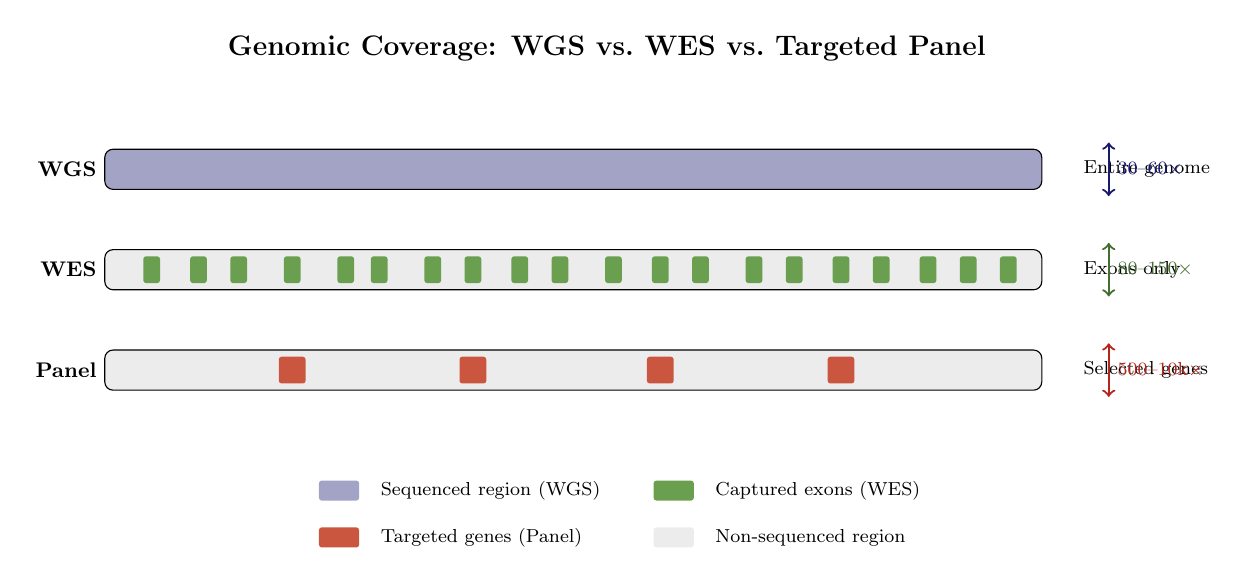
\begin{tikzpicture}[
  scale=0.85,
  transform shape,
  every node/.style={font=\small},
  chrombar/.style={draw, minimum height=0.6cm, rounded corners=3pt, inner sep=0pt},
  exonblock/.style={fill=OliveGreen!70, minimum height=0.4cm, rounded corners=1pt, inner sep=0pt},
  panelblock/.style={fill=BrickRed!70, minimum height=0.4cm, rounded corners=1pt, inner sep=0pt},
  label/.style={font=\small\bfseries, anchor=east},
]

% Title
\node[font=\large\bfseries, anchor=south] at (7, 7.5) {Genomic Coverage: WGS vs.\ WES vs.\ Targeted Panel};

% --- WGS ---
\node[label] at (-0.5, 6) {WGS};
\node[chrombar, fill=MidnightBlue!40, minimum width=14cm] at (6.5, 6) {};
\node[font=\footnotesize, anchor=west] at (14, 6) {Entire genome};

% --- WES ---
\node[label] at (-0.5, 4.5) {WES};
% Background chromosome
\node[chrombar, fill=gray!15, minimum width=14cm] at (6.5, 4.5) {};
% Exons scattered across
\foreach \x in {0.2, 0.9, 1.5, 2.3, 3.1, 3.6, 4.4, 5.0, 5.7, 6.3, 7.1, 7.8, 8.4, 9.2, 9.8, 10.5, 11.1, 11.8, 12.4, 13.0} {
  \node[exonblock, minimum width=0.25cm] at (\x, 4.5) {};
}
\node[font=\footnotesize, anchor=west] at (14, 4.5) {Exons only};

% --- Panel ---
\node[label] at (-0.5, 3) {Panel};
% Background chromosome
\node[chrombar, fill=gray!15, minimum width=14cm] at (6.5, 3) {};
% Only a few targeted genes
\foreach \x in {2.3, 5.0, 7.8, 10.5} {
  \node[panelblock, minimum width=0.4cm] at (\x, 3) {};
}
\node[font=\footnotesize, anchor=west] at (14, 3) {Selected genes};

% Legend
\node[fill=MidnightBlue!40, minimum width=0.6cm, minimum height=0.3cm, rounded corners=1pt] at (3, 1.2) {};
\node[anchor=west, font=\footnotesize] at (3.5, 1.2) {Sequenced region (WGS)};
\node[fill=OliveGreen!70, minimum width=0.6cm, minimum height=0.3cm, rounded corners=1pt] at (8, 1.2) {};
\node[anchor=west, font=\footnotesize] at (8.5, 1.2) {Captured exons (WES)};
\node[fill=BrickRed!70, minimum width=0.6cm, minimum height=0.3cm, rounded corners=1pt] at (3, 0.5) {};
\node[anchor=west, font=\footnotesize] at (3.5, 0.5) {Targeted genes (Panel)};
\node[fill=gray!15, minimum width=0.6cm, minimum height=0.3cm, rounded corners=1pt] at (8, 0.5) {};
\node[anchor=west, font=\footnotesize] at (8.5, 0.5) {Non-sequenced region};

% Depth annotations
\draw[<->, thick, MidnightBlue] (14.5, 5.6) -- (14.5, 6.4) node[midway, right, font=\footnotesize] {30--60$\times$};
\draw[<->, thick, OliveGreen!80!black] (14.5, 4.1) -- (14.5, 4.9) node[midway, right, font=\footnotesize] {80--150$\times$};
\draw[<->, thick, BrickRed] (14.5, 2.6) -- (14.5, 3.4) node[midway, right, font=\footnotesize] {500--10k$\times$};

\end{tikzpicture}
\caption{Visual comparison of genomic coverage achieved by whole-genome sequencing, whole-exome sequencing, and targeted gene panels. WGS covers the entire genome at moderate depth; WES selectively captures exonic regions at higher depth; targeted panels focus on a small gene set at very high depth.}
\label{fig:wgs_wes_panel}
\end{figure}

%% ============================================================
\section{Practical Bioinformatics: WGS Analysis Pipelines}
\label{sec:wgs_pipeline}
%% ============================================================

In this section, we build a complete WGS germline variant calling pipeline in both Snakemake and Nextflow. The workflow follows the best-practice GATK pipeline: quality control with \software{FastQC}, read trimming with \software{fastp}, alignment with \software{BWA-MEM2}, duplicate marking with \software{sambamba}, base quality score recalibration with \software{GATK}, variant calling with both \software{GATK HaplotypeCaller} and \software{DeepVariant}, and variant filtering.

\subsection{Snakemake WGS Pipeline}

\begin{lstlisting}[language=Python, caption={Complete Snakemake WGS germline variant calling pipeline.}, label={lst:snakemake_wgs}]
# Snakefile for WGS Germline Variant Calling Pipeline
# Follows GATK Best Practices

configfile: "config.yaml"

SAMPLES = config["samples"]
REF = config["reference"]
KNOWN_SITES = config["known_sites"]  # dbSNP, Mills indels

rule all:
    input:
        expand("results/vcf/{sample}.filtered.vcf.gz", sample=SAMPLES),
        expand("results/deepvariant/{sample}.dv.vcf.gz", sample=SAMPLES),
        "results/multiqc/multiqc_report.html"

rule fastqc:
    input:
        r1="data/fastq/{sample}_R1.fastq.gz",
        r2="data/fastq/{sample}_R2.fastq.gz"
    output:
        html1="results/qc/fastqc/{sample}_R1_fastqc.html",
        html2="results/qc/fastqc/{sample}_R2_fastqc.html",
        zip1="results/qc/fastqc/{sample}_R1_fastqc.zip",
        zip2="results/qc/fastqc/{sample}_R2_fastqc.zip"
    threads: 2
    shell:
        """
        fastqc -t {threads} -o results/qc/fastqc/ \
            {input.r1} {input.r2}
        """

rule fastp_trim:
    input:
        r1="data/fastq/{sample}_R1.fastq.gz",
        r2="data/fastq/{sample}_R2.fastq.gz"
    output:
        r1="results/trimmed/{sample}_R1.trimmed.fastq.gz",
        r2="results/trimmed/{sample}_R2.trimmed.fastq.gz",
        json="results/qc/fastp/{sample}.fastp.json",
        html="results/qc/fastp/{sample}.fastp.html"
    threads: 4
    shell:
        """
        fastp -i {input.r1} -I {input.r2} \
            -o {output.r1} -O {output.r2} \
            --json {output.json} --html {output.html} \
            --qualified_quality_phred 20 \
            --length_required 50 \
            --adapter_sequence auto \
            --thread {threads}
        """

rule bwa_mem2_align:
    input:
        r1="results/trimmed/{sample}_R1.trimmed.fastq.gz",
        r2="results/trimmed/{sample}_R2.trimmed.fastq.gz",
        ref=REF
    output:
        bam="results/aligned/{sample}.sorted.bam"
    params:
        rg="@RG\\tID:{sample}\\tSM:{sample}\\tPL:ILLUMINA\\tLB:lib1"
    threads: 16
    shell:
        """
        bwa-mem2 mem -t {threads} -R '{params.rg}' {input.ref} \
            {input.r1} {input.r2} \
        | samtools sort -@ 4 -o {output.bam} -
        samtools index {output.bam}
        """

rule sambamba_markdup:
    input:
        bam="results/aligned/{sample}.sorted.bam"
    output:
        bam="results/dedup/{sample}.dedup.bam",
        bai="results/dedup/{sample}.dedup.bam.bai"
    threads: 8
    shell:
        """
        sambamba markdup -t {threads} \
            --tmpdir tmp/ \
            {input.bam} {output.bam}
        """

rule gatk_bqsr:
    input:
        bam="results/dedup/{sample}.dedup.bam",
        ref=REF,
        known=KNOWN_SITES
    output:
        table="results/bqsr/{sample}.recal_data.table",
        bam="results/bqsr/{sample}.recal.bam"
    shell:
        """
        gatk BaseRecalibrator \
            -I {input.bam} -R {input.ref} \
            --known-sites {input.known} \
            -O {output.table}

        gatk ApplyBQSR \
            -I {input.bam} -R {input.ref} \
            --bqsr-recal-file {output.table} \
            -O {output.bam}
        """

rule gatk_haplotypecaller:
    input:
        bam="results/bqsr/{sample}.recal.bam",
        ref=REF
    output:
        gvcf="results/gvcf/{sample}.g.vcf.gz"
    threads: 4
    shell:
        """
        gatk HaplotypeCaller \
            -I {input.bam} -R {input.ref} \
            -O {output.gvcf} \
            -ERC GVCF \
            --native-pair-hmm-threads {threads}
        """

rule gatk_genotype:
    input:
        gvcf="results/gvcf/{sample}.g.vcf.gz",
        ref=REF
    output:
        vcf="results/vcf/{sample}.raw.vcf.gz"
    shell:
        """
        gatk GenotypeGVCFs \
            -R {input.ref} \
            -V {input.gvcf} \
            -O {output.vcf}
        """

rule gatk_filter:
    input:
        vcf="results/vcf/{sample}.raw.vcf.gz",
        ref=REF
    output:
        vcf="results/vcf/{sample}.filtered.vcf.gz"
    shell:
        """
        gatk VariantFiltration \
            -R {input.ref} -V {input.vcf} \
            --filter-expression "QD < 2.0" --filter-name "LowQD" \
            --filter-expression "FS > 60.0" --filter-name "StrandBias" \
            --filter-expression "MQ < 40.0" --filter-name "LowMQ" \
            --filter-expression "MQRankSum < -12.5" --filter-name "MQRankSum" \
            --filter-expression "ReadPosRankSum < -8.0" --filter-name "ReadPos" \
            -O {output.vcf}
        """

rule deepvariant:
    input:
        bam="results/dedup/{sample}.dedup.bam",
        ref=REF
    output:
        vcf="results/deepvariant/{sample}.dv.vcf.gz"
    threads: 16
    shell:
        """
        run_deepvariant \
            --model_type=WGS \
            --ref={input.ref} \
            --reads={input.bam} \
            --output_vcf={output.vcf} \
            --num_shards={threads}
        """

rule multiqc:
    input:
        expand("results/qc/fastqc/{sample}_R1_fastqc.zip", sample=SAMPLES),
        expand("results/qc/fastp/{sample}.fastp.json", sample=SAMPLES)
    output:
        "results/multiqc/multiqc_report.html"
    shell:
        """
        multiqc results/qc/ -o results/multiqc/ --force
        """
\end{lstlisting}

\subsection{Nextflow WGS Pipeline}

\begin{lstlisting}[language=Java, caption={Complete Nextflow DSL2 WGS germline variant calling pipeline.}, label={lst:nextflow_wgs}]
#!/usr/bin/env nextflow
nextflow.enable.dsl=2

// Nextflow WGS Germline Variant Calling Pipeline
// Follows GATK Best Practices

params.reads    = "data/fastq/*_{R1,R2}.fastq.gz"
params.ref      = "reference/hg38.fa"
params.known    = "reference/known_sites.vcf.gz"
params.outdir   = "results"

// ---- Processes ----

process FASTQC {
    tag "$sample_id"
    publishDir "${params.outdir}/qc/fastqc", mode: 'copy'
    cpus 2

    input:
    tuple val(sample_id), path(reads)

    output:
    path("*.{html,zip}"), emit: reports

    script:
    """
    fastqc -t ${task.cpus} ${reads}
    """
}

process FASTP {
    tag "$sample_id"
    publishDir "${params.outdir}/trimmed", mode: 'copy'
    cpus 4

    input:
    tuple val(sample_id), path(reads)

    output:
    tuple val(sample_id),
          path("${sample_id}_R{1,2}.trimmed.fastq.gz"),
          emit: trimmed_reads
    path("${sample_id}.fastp.{json,html}"),
          emit: reports

    script:
    """
    fastp -i ${reads[0]} -I ${reads[1]} \
        -o ${sample_id}_R1.trimmed.fastq.gz \
        -O ${sample_id}_R2.trimmed.fastq.gz \
        --json ${sample_id}.fastp.json \
        --html ${sample_id}.fastp.html \
        --qualified_quality_phred 20 \
        --length_required 50 \
        --thread ${task.cpus}
    """
}

process BWA_MEM2 {
    tag "$sample_id"
    publishDir "${params.outdir}/aligned", mode: 'copy'
    cpus 16

    input:
    tuple val(sample_id), path(reads)
    path ref
    path ref_idx  // .fai, .bwt.2bit.64, .amb, .ann, .pac

    output:
    tuple val(sample_id), path("${sample_id}.sorted.bam"),
          path("${sample_id}.sorted.bam.bai"),
          emit: aligned_bam

    script:
    """
    bwa-mem2 mem -t ${task.cpus} \
        -R "@RG\\tID:${sample_id}\\tSM:${sample_id}\\tPL:ILLUMINA\\tLB:lib1" \
        ${ref} ${reads} \
    | samtools sort -@ 4 -o ${sample_id}.sorted.bam -
    samtools index ${sample_id}.sorted.bam
    """
}

process SAMBAMBA_MARKDUP {
    tag "$sample_id"
    publishDir "${params.outdir}/dedup", mode: 'copy'
    cpus 8

    input:
    tuple val(sample_id), path(bam), path(bai)

    output:
    tuple val(sample_id), path("${sample_id}.dedup.bam"),
          path("${sample_id}.dedup.bam.bai"),
          emit: dedup_bam

    script:
    """
    sambamba markdup -t ${task.cpus} ${bam} ${sample_id}.dedup.bam
    """
}

process GATK_BQSR {
    tag "$sample_id"
    publishDir "${params.outdir}/bqsr", mode: 'copy'

    input:
    tuple val(sample_id), path(bam), path(bai)
    path ref
    path ref_fai
    path ref_dict
    path known_sites
    path known_sites_idx

    output:
    tuple val(sample_id), path("${sample_id}.recal.bam"),
          path("${sample_id}.recal.bam.bai"),
          emit: recal_bam

    script:
    """
    gatk BaseRecalibrator \
        -I ${bam} -R ${ref} \
        --known-sites ${known_sites} \
        -O ${sample_id}.recal_data.table

    gatk ApplyBQSR \
        -I ${bam} -R ${ref} \
        --bqsr-recal-file ${sample_id}.recal_data.table \
        -O ${sample_id}.recal.bam

    samtools index ${sample_id}.recal.bam
    """
}

process HAPLOTYPECALLER {
    tag "$sample_id"
    publishDir "${params.outdir}/vcf", mode: 'copy'
    cpus 4

    input:
    tuple val(sample_id), path(bam), path(bai)
    path ref
    path ref_fai
    path ref_dict

    output:
    tuple val(sample_id),
          path("${sample_id}.g.vcf.gz"),
          emit: gvcf

    script:
    """
    gatk HaplotypeCaller \
        -I ${bam} -R ${ref} \
        -O ${sample_id}.g.vcf.gz \
        -ERC GVCF \
        --native-pair-hmm-threads ${task.cpus}
    """
}

process DEEPVARIANT {
    tag "$sample_id"
    publishDir "${params.outdir}/deepvariant", mode: 'copy'
    cpus 16

    input:
    tuple val(sample_id), path(bam), path(bai)
    path ref
    path ref_fai

    output:
    tuple val(sample_id),
          path("${sample_id}.dv.vcf.gz"),
          emit: dv_vcf

    script:
    """
    run_deepvariant \
        --model_type=WGS \
        --ref=${ref} \
        --reads=${bam} \
        --output_vcf=${sample_id}.dv.vcf.gz \
        --num_shards=${task.cpus}
    """
}

process MULTIQC {
    publishDir "${params.outdir}/multiqc", mode: 'copy'

    input:
    path(reports)

    output:
    path("multiqc_report.html")

    script:
    """
    multiqc . -o . --force
    """
}

// ---- Workflow ----

workflow {
    // Create read-pair channel
    Channel
        .fromFilePairs(params.reads)
        .set { read_pairs_ch }

    ref          = file(params.ref)
    ref_fai      = file("${params.ref}.fai")
    ref_dict     = file(params.ref.replaceAll('.fa$', '.dict'))
    ref_idx      = Channel.fromPath("${params.ref}.*").collect()
    known_sites  = file(params.known)
    known_idx    = file("${params.known}.tbi")

    // Step 1: QC and trimming (in parallel)
    FASTQC(read_pairs_ch)
    FASTP(read_pairs_ch)

    // Step 2: Alignment
    BWA_MEM2(FASTP.out.trimmed_reads, ref, ref_idx)

    // Step 3: Duplicate marking
    SAMBAMBA_MARKDUP(BWA_MEM2.out.aligned_bam)

    // Step 4: BQSR
    GATK_BQSR(SAMBAMBA_MARKDUP.out.dedup_bam,
              ref, ref_fai, ref_dict,
              known_sites, known_idx)

    // Step 5: Variant calling (two callers in parallel)
    HAPLOTYPECALLER(GATK_BQSR.out.recal_bam,
                    ref, ref_fai, ref_dict)
    DEEPVARIANT(SAMBAMBA_MARKDUP.out.dedup_bam,
                ref, ref_fai)

    // Step 6: MultiQC report
    MULTIQC(
        FASTQC.out.reports
            .mix(FASTP.out.reports)
            .collect()
    )
}
\end{lstlisting}

\begin{tipbox}[title={Choosing Between Snakemake and Nextflow}]
Both workflow managers are widely used in genomics. Key considerations:
\begin{itemize}[nosep]
  \item \textbf{Snakemake}: Python-based, file-centric (rules define input/output files), integrates with Conda environments natively, excellent for bioinformaticians comfortable with Python.
  \item \textbf{Nextflow}: Groovy/Java-based, dataflow-driven (channels pass data between processes), strong Docker/Singularity integration, excellent for cloud-native and HPC deployments.
  \item \textbf{nf-core}: A community-curated collection of Nextflow pipelines. The \software{nf-core/sarek} pipeline implements a production-grade WGS/WES variant calling workflow with extensive QC and reporting.
\end{itemize}
\end{tipbox}

%% ============================================================
\section{Long-Read Alignment and Assembly Workflow}
\label{sec:longread_workflow}
%% ============================================================

For long-read WGS data, the alignment and variant calling tools differ:

\begin{itemize}[nosep]
  \item \textbf{Alignment}: \software{minimap2} with preset \texttt{-ax map-hifi} for PacBio HiFi or \texttt{-ax map-ont} for Oxford Nanopore.
  \item \textbf{Small variant calling}: \software{DeepVariant} (PacBio model or ONT model), \software{PEPPER-Margin-DeepVariant} for ONT, \software{Clair3}.
  \item \textbf{Structural variant calling}: \software{pbsv} (PacBio), \software{Sniffles2} (any long reads), \software{cuteSV}, \software{SVIM}.
  \item \textbf{Phasing}: \software{WhatsHap} for read-backed phasing, \software{HiPhase} for PacBio, \software{SHAPEIT5} for statistical phasing at population scale.
  \item \textbf{De novo assembly}: \software{hifiasm} for HiFi reads; \software{Verkko} for HiFi + ONT ultra-long; \software{Flye} for ONT-only assemblies.
  \item \textbf{Methylation}: \software{modkit} (PacBio), \software{modbam2bed} and \software{modkit} (ONT) for extracting base modification information.
\end{itemize}

%% ============================================================
\section{Quality Control Metrics for WGS/WES}
\label{sec:qc_metrics}
%% ============================================================

After alignment and before variant calling, it is essential to assess data quality. Key metrics include:

\begin{table}[htbp]
\centering
\caption{Essential QC metrics for WGS and WES data.}
\label{tab:qc_metrics}
\begin{tabularx}{\textwidth}{@{}lXl@{}}
\toprule
\textbf{Metric} & \textbf{Description} & \textbf{Typical Threshold} \\
\midrule
Mean coverage & Average number of reads covering each base & $\geq$30$\times$ (WGS) \\
\% bases $\geq$20$\times$ & Uniformity of coverage & $\geq$90\% \\
\% mapped reads & Fraction of reads aligning to reference & $\geq$95\% \\
\% properly paired & Fraction of read pairs with concordant alignment & $\geq$90\% \\
\% duplicate reads & PCR duplicate rate & $<$15\% (PCR-free: $<$5\%) \\
Insert size & Fragment length distribution (peak and spread) & 300--500\basepair{} \\
GC bias & Deviation of coverage across GC content bins & Minimal deviation \\
Contamination & Cross-sample contamination (VerifyBamID) & $<$1\% \\
Chimeric reads & Fraction of supplementary/split alignments & $<$5\% \\
On-target rate (WES) & Fraction of reads on capture target & $\geq$70\% \\
\bottomrule
\end{tabularx}
\end{table}

Tools for collecting these metrics include \software{samtools stats}, \software{Picard CollectWgsMetrics}, \software{Picard CollectHsMetrics} (for WES), \software{mosdepth} (fast coverage calculation), and \software{VerifyBamID2} (contamination estimation).

%% ============================================================
\section{Summary}
\label{sec:ch07_summary}
%% ============================================================

\begin{keyconcept}[title={Chapter Summary}]
\begin{itemize}[nosep]
  \item \textbf{WGS} captures the entire genome including coding, non-coding, regulatory, and repetitive regions. It is the most comprehensive but most expensive approach, requiring 30$\times$ for germline and 60--100$\times$ for somatic applications.
  \item \textbf{WES} captures $\sim$1--2\% of the genome (protein-coding exons) at a fraction of the cost of WGS. It is the workhorse for Mendelian disease diagnostics but misses non-coding and structural variants.
  \item \textbf{Targeted panels} offer ultra-deep sequencing of curated gene sets, ideal for clinical diagnostics with well-defined genetic targets.
  \item \textbf{Long-read WGS} (PacBio HiFi, Oxford Nanopore) enables structural variant detection, repeat characterisation, haplotype phasing, and de novo assembly---capabilities that are limited or absent with short reads alone.
  \item The \textbf{T2T-CHM13} assembly and emerging \textbf{pangenome references} are transforming how we represent and analyse human genetic variation.
  \item Both \textbf{Snakemake} and \textbf{Nextflow} provide robust frameworks for building reproducible WGS/WES analysis pipelines, with community-curated pipelines (e.g., \software{nf-core/sarek}) available for immediate use.
\end{itemize}
\end{keyconcept}
